	\newpage
\section{Ogólne określenie wymagań}		%1
%Określenie celu pracy, co chcemy uzyskać, jakie przewidujemy wyniki













\hspace{0.60cm}Tutaj może coś być wpisane. 

\subsection{Przykład}  %1.1       

\hspace{0.60cm}Tak zaczynamy pisanie pierwszego akapitu. Jeśli chcemy napisać przypis do bibliografii wykonujemy to w~ten sposób\footnote{Przykład odnośnika do książki\cite{legierski}.}.

%rysunek
	\begin{figure}[!htb]
	\begin{center}
		
\includegraphics[width=8cm]{rys/ans.png}
		\caption{Logo}
		\label{rys:rysunek001}
	\end{center}
\end{figure}

\fg{rys/ans.png}{Logo}{rys:rysunek003}

Tutaj może coś być wpisane. \\Tutaj może coś być wpisane\footnote{Przykład odnośnika do strony www\cite{www1}.}. 
Rysunek \ref{rys:rysunek001} (s. \pageref{rys:rysunek001}) pokazuje przykładową ilustrację.

%tabelka
\begin{tabela}
	%uwaga: w nawiasach [] nie może być odnośnika do literatury, jeżeli w dokumencie jest spis rysunków na początku, a spis literatury jest w kolejności cytowania (zmienia to numeracji)
	{Tabelka przykładowa}	%opis w spisie tabel
	{Tabelka przykładowa}	%opis przy tabeli
	{
		\begin{tabular}{|c|c|} \hline
			$U_n$ & $I_{zw}$ \\ \hline
			$kV$  & $\%$      \\ \hline
			7.2 & 100 \\ \hline
		\end{tabular}
	}
	\label{tab:tablica001}
\end{tabela}

% Kod

Listing kodu

\begin{lstlisting}[caption=Przykładowy kod 001, label={lst:listing-cpp}, language=C++]
#include <iostream>
#include <cstdlib>
#include <ctime>
using namespace std;

/*
liczby pseldolosowe
*/

int main(int argc, char** argv) {
	
	int tab[10][10];
	
	for(int i=0;i<10;i++)
	for(int j=0;j<10;j++)
	tab[i][j]=0;
	
	srand(time(NULL));		//generowanie z czasu
	int min=3;
	int max=7;
	for(int i=0;i<10;i++)
	for(int j=0;j<10;j++)		
	tab[i][j]=(rand()%(max-min+1))+min;	
	
	for(int i=0;i<10;i++)
	{
		for(int j=0;j<10;j++)
		cout<<tab[i][j]<<" ";	
		cout<<endl;
	}
	
	return 0;
}
\end{lstlisting}

Tutaj może coś być wpisane. Tutaj może coś być wpisane. Tutaj może coś być wpisane. Tabela \ref{tab:tablica001} (s. \pageref{tab:tablica001}) pokazuje sposoby użycia trybu matematycznego.

Kod \ref{lst:listing-cpp} (s. \pageref{lst:listing-cpp}) przedstawia sposób generowania liczb pseudolosowych. Kod \ref{lst:listing-cpp2} (s. \pageref{lst:listing-cpp2}) przedstawia generowanie pliku HTML.

Alternatywna metoda wklejenia kodu:

\lstinputlisting[caption=Przykładowy kod 002, label={lst:listing-cpp2}, language=C++]{kod/main.cpp}


\subsection{Instalacja}  %1.2

\hspace{0.60cm}Poniżej są opisane kroki potrzebne do instalacji \LaTeX 'a oraz do używania tego szablonu.

 Na początku instalujemy \TeX{}Live\footnote{Instalka na stronie  https://www.tug.org/texlive/acquire-netinstall.html\cite{www2}.}. Ściągamy plik instalacyjny, zajmuje około 25MB. Podczas instalacji można wybrać do zainstalowania różne kolekcje pakietów. Jeśli nie ma problemów z miejscem na dysku to można zainstalować wszystkie, wtedy nie będzie problemu z brakującymi pakietami i błędami. Po wybraniu kolekcji brakujące pliki są pobierane z internetu. Pełna instalacja programu zajmuje około 8GB. Najlepiej zostawić instalację na noc, ponieważ proces zabiera sporo czasu. Warto ustawić komputer tak, aby się nie wyłączył lub nie uśpił. Warto także przed instalacją zablokować antywirusa, ponieważ może blokować niektóre z komponentów.
 
Następnie instalujemy \TeX{}studio\footnote{Plik instalacyjny na stronie  https://www.texstudio.org\cite{www3}.}. Ściągamy plik instalacyjny zajmujący około 120MB. Instalacja przebiega standardowo.

 %rysunek
\begin{figure}[!hbt]
	\begin{center}
		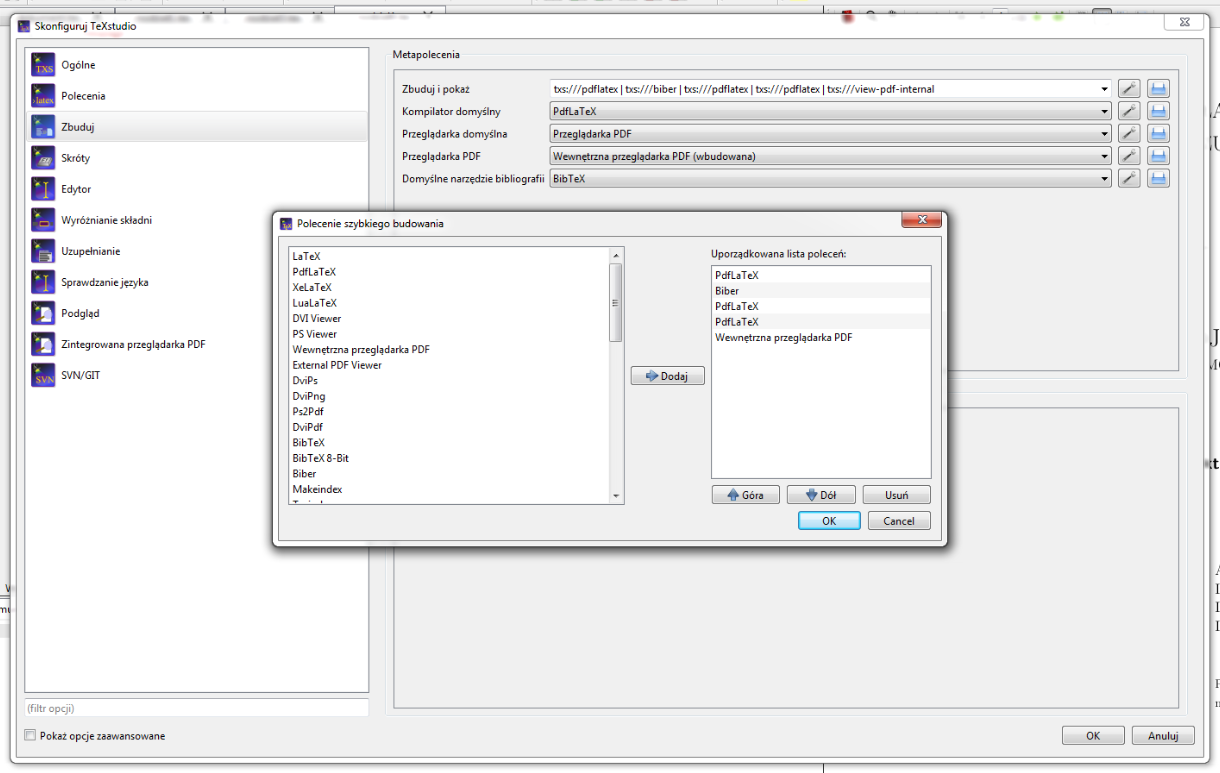
\includegraphics[width=\linewidth]{rys/ustawienie.png}
		\caption{Ustawienie TeXstudio}
		\label{rys:ustawienia}
	\end{center}
\end{figure}

Następnym krokiem jest ustawienie w \TeX{}Studio kolejności budowania projektu. Należy wybrać zakładkę: ,,Opcje/Konfiguruj \TeX{}studio...''. W otwartym oknie przechodzimy na zakładkę ,,Zbuduj''. Na rysunku \ref{rys:ustawienia} (s. \pageref{rys:ustawienia}) pokazany jest zrzut ekranu z konfiguracją. W linijce ,,Zbuduj i pokaż'' klikamy ikonę klucza, żeby przejść do konfiguracji polecenia. W otwartym oknie ustawić kolejność tak jak pokazano na rysunku.

 
 
 
 
 